\documentclass[tikz,border=10pt]{standalone}
\usepackage{tikz}
\usetikzlibrary{arrows.meta,positioning,calc}

\begin{document}
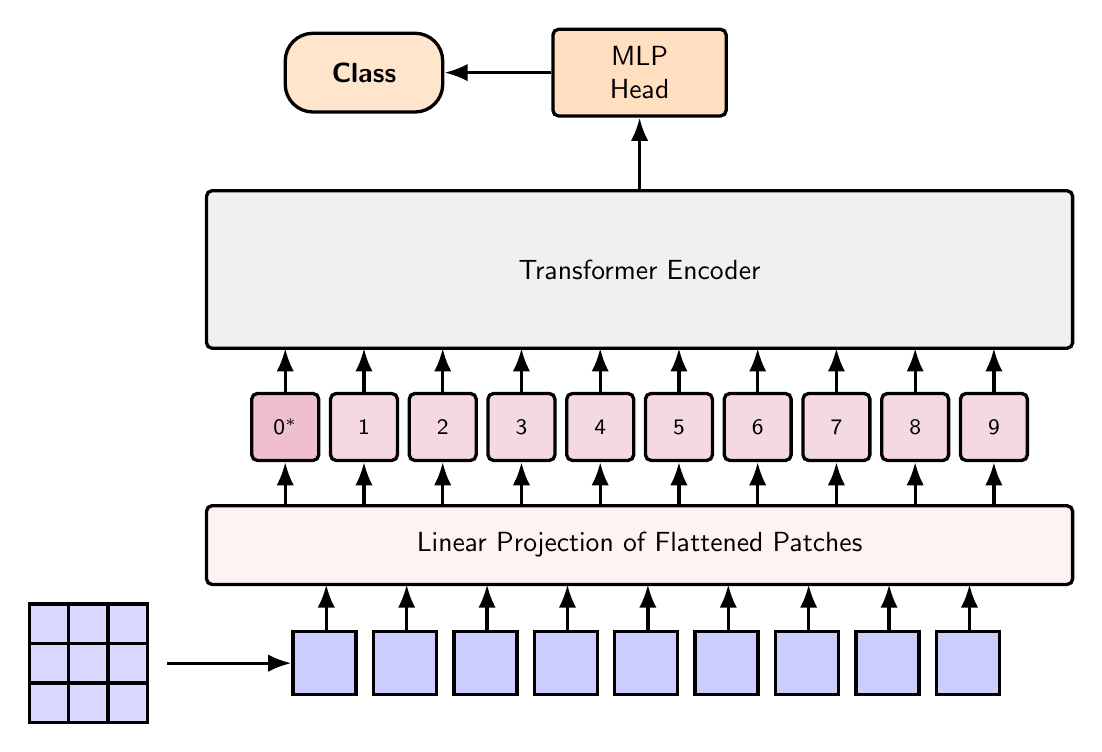
\begin{tikzpicture}[
  font=\sffamily,
  >=Latex,
  thick,
  box/.style={draw, rounded corners=2pt, very thick, align=center, minimum height=10mm, fill=gray!12},
  head/.style={draw, rounded corners=2pt, very thick, align=center, minimum height=11mm, minimum width=22mm, fill=orange!25},
  token/.style={draw, rounded corners=2pt, very thick, minimum height=8.5mm, minimum width=8.5mm, fill=purple!15, align=center},
  tokencls/.style={token, fill=purple!25},
  patch/.style={draw, very thick, minimum size=8mm, fill=blue!20},
  patch2/.style={draw, very thick, minimum size=8mm, fill=green!20},
  proj/.style={box, fill=pink!20, minimum height=10mm},
  enc/.style={box, minimum height=20mm, minimum width=110mm},
  bubble/.style={draw, very thick, rounded corners=10pt, fill=orange!20, align=left, minimum width=20mm, minimum height=10mm}
]


\def\patchsep{6.0mm}     % パッチ間隔（大きく）

%========================
% Class output bubble
%========================
\node[bubble] (classbubble) at (2.0,7.5) {\bfseries Class};

%========================
% Transformer Encoder + MLP head
%========================
\node[enc] (encMain) at (5.5,5.0) {Transformer Encoder};
\node[head] (mlpHead) at (5.5,7.5) {MLP\\Head};

\draw[->,very thick] (encMain.north) -- (mlpHead.south);
\draw[->,very thick] (mlpHead.west) -- (classbubble.east);

%========================
% Tokens row
%========================
\coordinate (tokBase) at (1.0,3.0);

\node[tokencls] (t0) at (tokBase) {\footnotesize 0$^\ast$};
\foreach \i in {1,...,9}{
    \node[token] (t\i) at ($(tokBase)+(\i*1.0,0)$) {\footnotesize \i};
}

% Arrows from tokens to encoder (vertical arrows)
\foreach \i in {0,...,9}{
    \draw[->,very thick] (t\i.north) -- ($(1+\i,4)$);
}

%========================
% Linear Projection box
%========================
\node[proj, minimum width=110mm] (linproj) at (5.5,1.5) {Linear Projection of Flattened Patches};

%========================
% Patch thumbnails row (under projection)
%========================
\coordinate (prow) at (1.5,0.0);
\node[patch]  (p1) at (prow) {};
\node[patch] (p2) at ($(p1.east)+(\patchsep,0)$) {};
\node[patch]  (p3) at ($(p2.east)+(\patchsep,0)$) {};
\node[patch] (p4) at ($(p3.east)+(\patchsep,0)$) {};
\node[patch]  (p5) at ($(p4.east)+(\patchsep,0)$) {};
\node[patch] (p6) at ($(p5.east)+(\patchsep,0)$) {};
\node[patch]  (p7) at ($(p6.east)+(\patchsep,0)$) {};
\node[patch] (p8) at ($(p7.east)+(\patchsep,0)$) {};
\node[patch]  (p9) at ($(p8.east)+(\patchsep,0)$) {};

% Arrows: linear projection -> tokens (one per token)
% （射影の上端からトークンへ、横方向に余裕を持って分配）
\foreach \i in {0,...,9}{
  \draw[->,very thick]
    ($(\i+1,2)$) -- (t\i.south);
}

% Arrow: patch thumbnails -> linear projection
% \draw[->,very thick] ($(p5.north)+(0,2.0mm)$) -- (linproj.south);
\foreach \i in {1,...,9}{
    \draw[->,very thick] ($(p\i.east)+(-0.4,0.4)$) -- ($(p\i.east)+(-0.4,1)$);
}


%========================
% Small patch grid (image split)
%========================
\coordinate (grid) at (-2.0,-0.5);
\foreach \x in {0,1,2}{
  \foreach \y in {0,1,2}{
    \node[patch, fill=blue!15, minimum size=5mm] at ($(grid)+(\x*5mm,\y*5mm)$) {};
  }
}

% Arrow: grid -> patch thumbnails row
\draw[->,very thick] (-0.5,0) -- (p1.west);

\end{tikzpicture}
\end{document}
